\documentclass[../report.tex]{subfiles}
\graphicspath{{\subfix{../image/}}}

\begin{document}
\maketitle

\section*{Introduction}

One of the main focuses of this third semester project is analog electronics. Electronics bring the software and the mechanical part together. 
The software needs feedback from the analog world. It needs to know how heavy the load is and
whether there is an obstacle in front. Furthermore, all the smart digital electronics need to be powered. 
But when powering everything from a battery the current state of the battery has to be evaluated.
All these tasks are necessary to guarantee safe operations.

\quad
The tasks include the following:

\begin{itemize}
    \item Interfacing the analog load cells
    \begin{itemize}
      \item Loadcell PCB Design
    \end{itemize} 
    \item Power Supply and monitoring
    \item \begin{itemize}
      \item VeroBoard Design
    \end{itemize}
    \item Motor Drivers
    \begin{itemize}
      \item Motor Driver PCB Design
    \end{itemize}  
\end{itemize}

\begin{figure}[h!]
  \centering
  \begin{subfigure}[b]{0.4\linewidth}
    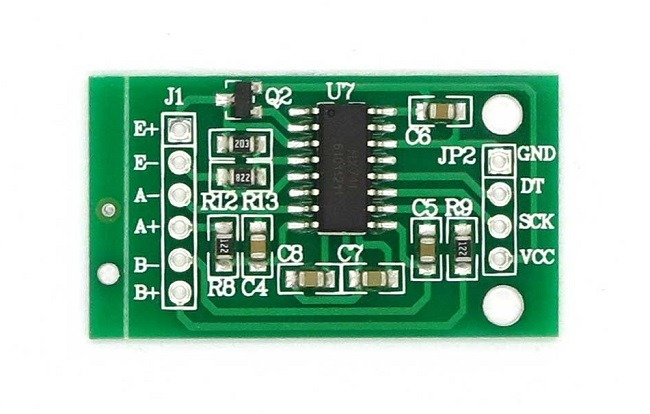
\includegraphics[width=\linewidth]{image/HX711-Weighing-Sensor-Dual-Channel-24-Bit-Precision-A-D-Module-Pressure-Sensor_1.jpg}
    \caption{HX711 Interface Module }
  \end{subfigure}
  \begin{subfigure}[b]{0.4\linewidth}
    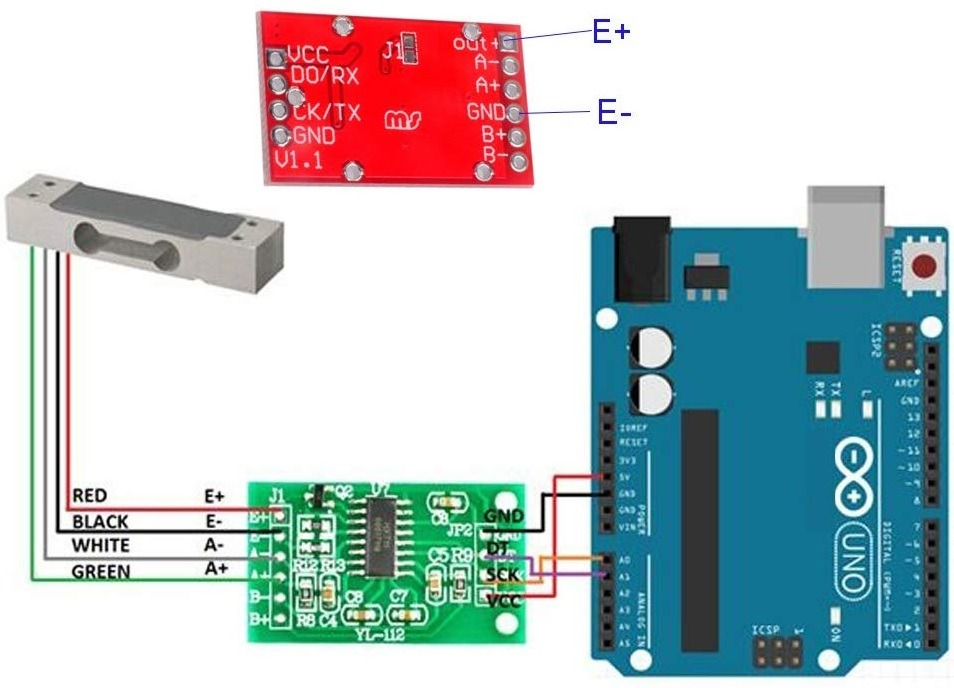
\includegraphics[width=\linewidth]{image/hx711-red.jpg}
    \caption{HX711 Interface Module and Load cell using Arduino-microcontroller}
  \end{subfigure}
  
  
\end{figure}
  
\end{document}